\chapter{Oppsummering}
I dette kapittelet oppsummeres våre erfaringer fra prosessdelen av EiT.
Vi går gjennom både individuelle- og grupperefeleksjoner.

\section{Individuelle refleksjoner}
\label{individuellerefleksjoner}
De individuelle refleksjonene forteller om erfaringene hvert enkelt gruppemedlem
har gjort seg gjennom dette halvåret.

\subsection*{Erlend Aksnes}
I dette prosjektet har jeg vært ganske lik meg i selv, litt tilbakeholden og redd for å ta ansvar, men til tider har jeg vært litt mer frempå og prøvd å ta litt mer ansvar. Store deler av prosjektet var knyttet til fagfelt jeg ikke kan noe særlig om, og jeg måtte derfor stole på de andre gruppemedlemmene. Siden jeg oppfattet de andre gruppemedlemmenes faglige nivå som høyt, hadde jeg ikke noe problem med å stole på dem. Dette var egentlig ikke en ny opplevelse for meg, da jeg har vært borti lignende tilfeller før ved store prosjektarbeid hvor man må dele opp oppgaven og stole på at de andre i gruppen klarer oppgaven sin. 

Prosessbiten har til tider vist seg å være kjedelig, men jeg synes samtidig at dette var svært lærerikt til tider. Jeg har lært meg å reflektere over situasjoner som oppstår gjennom arbeidsdagen, og er nå mer bevisst på hvordan jeg påvirker de andre i gruppen, samt hvordan de påvirker meg. Dette er absolutt noe jeg kommer til å ta med meg videre i fremtidige gruppearbeid, i både studiet og arbeidslivet.

Jeg ser tilbake på prosjektet som en lærerik prosess, hvor jeg har lært mest om gruppearbeid. De andre gruppemedlemmene har vært åpne for forslag gjennom hele prosjektet og jeg føler at alle har fått sine meninger og synspunkter vurdert på lik linje. Til tross for hva venner og bekjente hadde fortalt meg i forkant av EiT, opplevde jeg EiT som et av prosjektarbeidene jeg er mer fornøyde med. 

\subsection*{Emil Bjørlykhaug}
Kanskje det aller viktigste jeg sitter igjen med etter EiT er at folk kan tolke situasjoner og kommunikasjon ganske forskjellig, mye mer enn jeg før hadde trodd. Det er viktig å si i fra om en tror en tolker noe ulikt fra de andre, samtidig som det er viktig å prøve å være så tydelig som mulig når en kommuniserer. Misforståelser og mistolkninger kan føre til mer misnøye enn en kanskje skulle tro ved første øyekast. En annen ting jeg la merke til er hvor nært knyttet prosjekt og prosess er – uten noe handfast å jobbe med kan moralen i gruppen dale fort. Jeg har derfor nå en enda større forståelse for viktigheten av å fordele oppgaver, og at alle sitter med følelsen av at de gjør noe matnyttig.

Disse erfaringene føler jeg gjør at jeg stiller sterkere som et gruppemedlem nå, enn før EiT. EiT har gjort meg mer åpen til å stille spørsmål for å faktisk forstå hva som blir sagt, samtidig som jeg har større tiltro på mine evner på mitt fagfelt. 

\subsection*{David Hovind}
Eksperter i team har vært en helt annen opplevelse enn det jeg hadde forventet. 
Jeg trodde at vi skulle samles en gruppe med studenter med forskjellig bakgrunn, og sammen utvikle en prototype til et produkt eller noe. 
Tidlig i semesteret fant jeg ut at mesteparten av faget egentlig gikk ut på samarbeidet i gruppa, og det var ikke selve produktet som var viktig, men selve prosessene rundt det. 
Det var litt kjedelig til å begynne med, siden det var mye reflektering og ikke mye faktisk produktiv jobbing. 
Dette er noe jeg ikke var vant med fra før og jeg syntes ikke det var spesielt gøy eller nyttig heller.

Etterhvert utover semesteret begynte jeg å skjønne hvorfor vi hadde refleksjoner og slikt. 
Tidligere har jeg ikke vært med i tverrfaglige grupper, men når det var tilfellet nå så oppstod det noen konflikter. 
Selv er jeg konfliktsky, men jeg så at ved å reflektere over og være åpne om det som hadde skjedd og hvordan vi følte, så kunne vi faktisk komme fram til en løsning alle kunne være fornøyde med. 
Jeg tror også at mye av de konfliktene og uenighetene som oppstod, oppstod på grunn av prosessdelen av faget og det faktum at ingen av oss hadde noen særlig erfaring med det fra før. 

Jeg går ut av dette faget med nye og nyttige erfaringer. Jeg ser nå at for store prosjekter med tverrfaglig bakgrunn, kan det være lurt med en form for refleksjon for å løse opp i konflikter og situasjoner. 
Ofte så er det en del misforståelser, hvor folk tolker ting forskjellig, og dette kan fort skape konflikter og dårlig stemning.
Jeg har lært at jeg selv kan være litt tilbakeholden når det gjelder å gi kritikk til andre, og jeg prøver som regel å børste problemer litt under teppet.
Jeg er også litt dårlig til å motta kritikk, hvor jeg fort tar ting litt for mye innover meg selv, når det egentlig er ment som hjelpsomt og ikke slemt.
Alt i alt er jeg glad for at jeg hadde faget og jeg føler meg tryggere på hvordan gruppearbeid fungerer og hvordan jeg fungerer i gruppearbeid.

\subsection*{Kristoffer Løvall}
Det som har skilt seg ut med dette gruppearbeidet for min del, er at vi endte opp som en gruppe med flat struktur. Jeg hadde som mål i starten av 
semesteret å holde meg litt unna lederrollen, og synes det har fungert overraskende godt. I tillegg til at jeg selv pleier å ta på meg en lederrolle, har 
jeg oppfattet både Christoffer og til tider Nina som naturlige ledertyper, og ettersom vi er flere i gruppen med disse egenskapene, føltes det helt 
naturlig å fordele alle beslutninger og alt ansvar jevnt. Jeg har merket at det å ha et noe mer avslappet forhold til gruppearbeid enn tidligere, har 
fungert godt med tanke på effektivitet, og det å stole på en gruppe mennesker jeg nettopp har møtt til å fullføre en oppgave på en 
tilfredsstillende måte. Dette kan gjerne være fordi gruppen har holdt et veldig høyt faglig nivå, og ettersom jeg er den eneste på gruppen med 
maskinfaglig bakgrunn har jeg ikke hatt andre personer å ``sparre'' med innen mitt fagfelt. Som tidligere nevnt har jeg vært klar over at jeg kan bli 
noe kontrollerende i engasjerte øyeblikk, men denne (dårlige) egenskapen har jeg klart å holde i sjakk under arbeidet med EiT. 

Et annet aspekt som 
har overrasket positivt er selve refleksjonsbiten. Det var uten tvil en utfordring for meg, og andre i gruppen, å dele tanker og meninger på en 
såpass åpen måte med ukjente mennesker i oppstartsfasen. Etter hvert som vi kom litt mer inn i det, har det vist seg at det ikke bare i dette 
gruppearbeidet, men også i andre parallelle fag med gruppearbeid, har skapt et mye bedre samarbeid på et faglig så vel som sosialt plan. Jeg vil 
uten tvil ha et større fokus på meg selv for kommende gruppearbeid, altså på hvordan jeg oppfører meg ovenfor gruppen, og mindre på hvordan 
gruppen oppfører seg ovenfor meg.

\subsection*{Christoffer Ramstad-Evensen}
Etter å ha fullført EiT er inntrykkene jeg sitter igjen med positive. Ja, vi har innad i gruppen hatt våre utfordringer
på veien til hit vi er i dag, men totalt sett har vi fullført dette faget sammen. Når jeg sier dette er det for å rette 
fokuset på at læringsutbytte i denne perioden har vært stort. Noen elementer i læringen som har funnet sted
har vært selvsagte, men av og til trenger man å få det repetert. I tillegg er det som jeg nevnte innledningsvis
i introduksjonen en erfaring ved å jobbe i et team som man ikke kan få nok av. Jeg har også lært noen 
definisjoner jeg ikke skulle vært foruten samt forstått viktigheten av og ha en form for ledelse i et team. 
Vi har under hele EiT jobbet som et team uten leder, og det har gått greit, men arbeidet blir først fremprovosert
når noen tar ansvar og setter prosessen i gang. 

I tidlig fase av EiT syntes jeg oppsettet var ganske kunstig. Det var en situasjon jeg ikke kunne se for meg
finne sted i et reelt arbeidsmiljø. Vi hadde hele tiden veldig fokus på å evaluere hver eneste tanke og ord som
skulle deles i fellesskap. Dette førte til en del unødvendige småkonflikter og kommunikasjonen ble lite direkte. 
Allikevel tror jeg at det må være kunstig på denne måten for å fremprovosere situasjoner man kan ta lærdom av.

Jeg føler jeg tar med med mye positivitet og gode erfaringer fra dette faget og stiller sterkere i teamarbeid hos
fremtidige arbeidsgivere.

\subsection*{Nina Margrethe Smørsgård}
Etter å ha jobbet med EiT i et halvår nå, sitter jeg igjen med blanda følelser. 
Jeg vet fra før at jeg liker godt å jobbe målretta med et håndfast prosjekt, men jeg 
har merket at jeg har hatt veldig lite tålmodighet med prosessdelen. For 
min del ble arbeidsoppgavene i begynnelsen veldig vage, og det ble veldig passivt.

Jeg er av natur en person som ikke liker å tenke og føle så mye på det som skjer 
rundt meg, men heller jobber godt med håndfaste ting. Det betyr ikke at jeg ikke ser 
nytten av refleksjoner og evalueringer slik det er blitt gjort i EiT, jeg ser det 
bare som en veldig unaturlig og kunstig måte å tvinge det fram på, og dermed ser 
jeg ikke hvordan det kan overføres til en reell arbeidssituasjon.

Jeg tror grunnen til at jeg etterhvert ble så negativ til prosessdelen av EiT 
er at det ble så mye prosess i starten, men jeg vet ikke om det hadde vært bedre å få 
det fordelt litt og litt utover hele semesteret. Generelt sett mener jeg det er 
bedre å rive av plasteret ``fort og gæli'', og det gjør vondt der og da, men 
da der det også mye raskere over. 
På den annen side har jeg lært at folk oppfatter og forstår ting på forskjellig måte ut fra 
hvilken bakgrunn de har, og hvilken type kommunikasjon de er vante med fra før.
Jeg har en tendens til å kaste ut ganske harde ord og uttrykk, og har nok 
derfor blitt misforstått som noe mer negativ enn jeg faktisk har vært. 

\section{Grupperefleksjoner}

Gruppen føler at samarbeidet under EiT har vært interessant på mange måter. Sammen har vi måttet lære
hverandre å kjenne og hvordan vi skal kunne jobbe sammen på best mulig måte. Konfliktene har ikke vært få,
men de har gitt oss en god erfaring til nye teamsamarbeid. Det er i midt oppe i disse konfliktene vi har fått
utforsket hvordan man selv som person påvirker et teamarbeid og fått oppleve hvor ulike mennesker kan være. 


Figurene under viser samarbeidsindikatoren basert på resultatene i den første spørreundersøkelsen, figur \ref{fig:si1},
og samarbeidsindikatoren basert på resultatene i den siste spørreundersøkelsen i semesteret, figur \ref{fig:si2}.
\begin{figure}[H] \centering
\subfigure[]{
	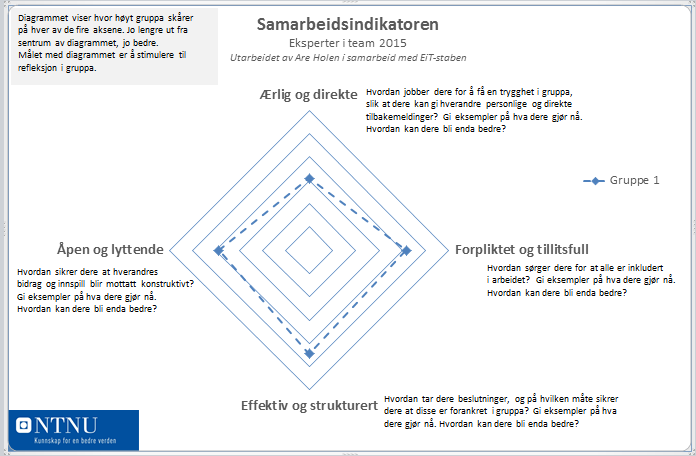
\includegraphics[width=0.60 \textwidth]{images/samarbeidsindikator_1.png}
	\label{fig:si1}
	}
\subfigure[]{
	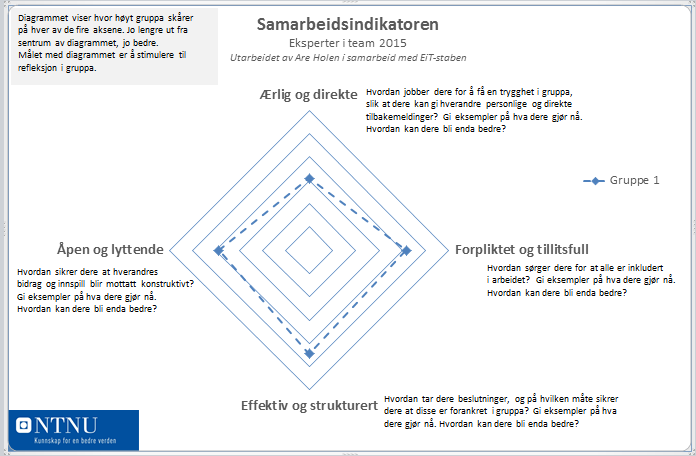
\includegraphics[width=0.60 \textwidth]{images/samarbeidsindikator_2.png}
	\label{fig:si2}
	}
\caption{Samarbeidsindikatorer: \protect{\ref{fig:si1}} første spørreundersøkelse, \protect{\ref{fig:si2}} siste spørre{-}undersøkelse.}
\end{figure}
Som man ser av sammenligningen av disse resultatene, gjengitt i figur \ref{fig:si3}, 
har vi blitt mer åpne og lyttende, samt mer ærlige og direkte.
Vi føler at disse resultatene er representative for utviklingen, 
og stemmer overens med hvordan vi selv ser på utviklingen i gruppen. 
	\newline
	\begin{figure}[H]
		\centering
		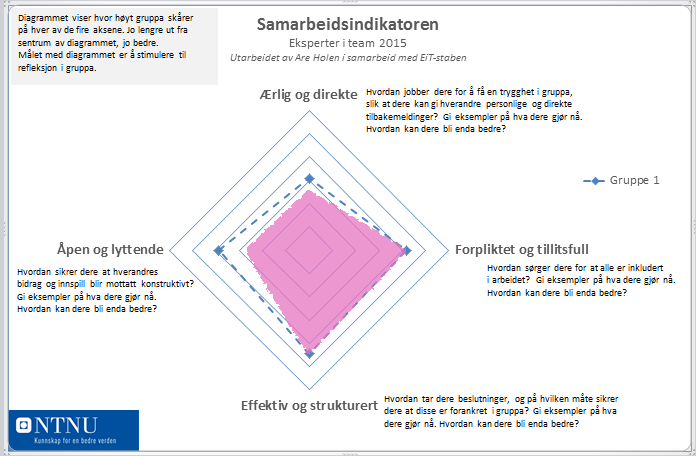
\includegraphics[width=1.00\textwidth]{images/samarbeidsindikator_sammenligning.png}
		\caption{Overlapp av resultatene fra første spørreundersøkelse (rosa), figur \ref{fig:si1}, og siste spørreundersøkelse, figur \ref{fig:si2}.}
		\label{fig:si3}
	\end{figure}

Vi mener grunnen til denne forbedringen er at vi har hatt fokus på å være mer direkte og mer presis i tilbakemeldinger.
Gruppen innså at for uklare tilbakemeldinger førte til misforståelser som førte til at stemningen i teamet ble anspent og fremdriften ble
svekket. Gjennom samarbeidet har vi utviklet oss som konfliktløsere, og vi har gått fra å være todelte på enkelte områder
til så å stå sammen som et enhetlig team.